\documentclass[pdflatex,sn-mathphys-num]{sn-jnl}

\usepackage{amsmath}
\usepackage{booktabs}
\usepackage{graphicx}
\usepackage{xcolor}
\graphicspath{{figures/}}
\renewcommand{\orcidlogo}{\hspace{.2em}\raisebox{.02em}{
\includegraphics[height=.69em]{orcid_mark.png}}}
\newif\ifformalsites
\IfFileExists{figures/formal_sites.pdf}{\formalsitestrue}{%
  \IfFileExists{formal_sites.pdf}{\formalsitestrue}{}}
\newcommand{\showtrialsequence}[1]{%
  \begin{figure}[htbp]
    \centering
    \includegraphics[width=\linewidth]{#1.pdf}
    \caption{Recorded views and wheel-odometry path for the indicated formal trial. Times are measured from the start of the recording. The lettered markers identify the nearest odometry samples in recorder time, relative to the first plotted pose. The path axes are scaled independently}
    \label{fig:#1}
  \end{figure}}
\newcommand{\loadtrialsequence}[1]{%
  \IfFileExists{figures/#1.pdf}{\showtrialsequence{#1}}{%
    \IfFileExists{#1.pdf}{\showtrialsequence{#1}}{}}}

\newif\ifdraftreview
\ifdefined\JINTAuthorReview\draftreviewtrue\fi
\definecolor{reviewink}{HTML}{784100}
\definecolor{reviewfill}{HTML}{FFF1D6}
\definecolor{overviewink}{HTML}{173852}
\newcommand{\reviewbadge}[1]{%
  \colorbox{reviewfill}{\textcolor{reviewink}{\sffamily\bfseries\strut #1}}}
\newcommand{\reviewlink}[2]{\hyperref[#1]{\textcolor{overviewink}{\underline{#2}}}}
\newcommand{\pending}[2]{%
  \ifdraftreview
    \hyperlink{author-checklist}{\reviewbadge{#1}}\nobreak\space
    \textcolor{reviewink}{\textbf{[Pending: #2]}}%
  \fi}
\newcommand{\vlidar}{V-LiDAR}
\newcommand{\m}{\,\mathrm{m}}

\begin{document}

\title[\vlidar{} for indoor obstacle avoidance]{V-LiDAR: Monocular Virtual Scans for Reactive Obstacle Avoidance in Structured Indoor Environments}
\subtitle{Categories (3), (6), (7)}

\author[1]{\fnm{Hyunwoo} \sur{Gu}\orcid{https://orcid.org/0009-0008-2779-648X}}
\author[1]{\fnm{Gunmin} \sur{Yoo}\orcid{https://orcid.org/0009-0001-6453-8075}}
\author[1]{\fnm{Hyunseo} \sur{Lee}\orcid{https://orcid.org/0009-0004-8217-7201}}
\author[1]{\fnm{Hyunmo} \sur{Kang}\orcid{https://orcid.org/0009-0004-7846-649X}}
\author[1]{\fnm{Minseok} \sur{Lee}}
\author*[1]{\fnm{Sung Soo} \sur{Hwang}\orcid{https://orcid.org/0000-0002-0863-7503}}\email{sshwang@handong.edu}
\affil[1]{\orgdiv{School of Artificial Intelligence, Computer and Electrical Engineering},
\orgname{Handong Global University}, \orgaddress{\city{Pohang}, \postcode{37554}, \country{Republic of Korea}}}

\abstract{Floor segmentation identifies traversable image regions for mobile robot obstacle avoidance. Using these regions in a navigation costmap requires an estimate of metric geometry and stable observations over time. This paper presents V-LiDAR, a monocular pipeline that projects visible ground-contact boundaries into a planar virtual scan for the Robot Operating System 2 Navigation2 stack. A calibrated lookup table estimates range and bearing from image coordinates, and temporal filtering stabilizes individual scan channels. The OpenVINO perception wrapper averaged 13.49 ms per frame in an offline onboard CPU benchmark. We define a repeatable avoidance protocol for a wheeled robot. It uses marked 10 m routes at three sites under four conditions and records physical goal arrival, contact, and manual intervention. In two exploratory bridge runs, the robot passed a stationary obstacle and the navigation stack reported arrival. Subsequent runs exposed planning difficulties and stale wheel feedback, motivating a reset and data-validation procedure. \ifdraftreview\hyperlink{author-checklist}{\reviewbadge{R4}}\space\fi The study focuses on structured, approximately planar environments and examines the operating limits imposed by reflections, incomplete floor masks, and near-field visibility.}

\keywords{Monocular vision, Virtual scan, Floor segmentation, Mobile robot, Obstacle avoidance, ROS 2}
\pacs[MSC Classification]{68T40, 68T45}

\maketitle
\raggedbottom

\ifdraftreview
\clearpage
\hypertarget{author-checklist}{}
{\Large\sffamily\bfseries\textcolor{overviewink}{Author review checklist}\par}
\smallskip
\noindent Internal working draft. Select a manuscript location below to jump to it. The amber tags in the text return to this page.
\medskip

\begingroup
\small
\renewcommand{\arraystretch}{1.35}
\setlength{\tabcolsep}{4pt}
\noindent\begin{tabular}{@{}lp{.24\linewidth}p{.60\linewidth}@{}}
\toprule
ID & Needed & Evidence and manuscript location \\
\midrule
\reviewbadge{R1} & Field records & Verify physical goal arrival, contact, and intervention for the four conditions. Match observer records to the bags and outcome logs. \reviewlink{sec:evaluation}{Evaluation protocol} \\
\reviewbadge{R2} & Deployed setup & Confirm the camera and scan frames, firmware, model, lookup table, costmap, and trial limits actually used. \reviewlink{sec:deployed-setup}{Navigation integration} \\
\reviewbadge{R3} & Training provenance & Recover the dataset version, class mapping, annotation procedure, and split counts. \reviewlink{sec:floor-segmentation}{Floor segmentation} \\
\reviewbadge{R4} & Results and claims & Summarize verified outcomes by condition and layout, document representative success and failure, and revise the abstract and conclusion. \reviewlink{sec:formal-outcomes}{Formal outcomes} \textperiodcentered{} \reviewlink{sec:discussion}{Discussion} \\
\reviewbadge{R5} & Author declarations & The author list, corresponding author, and equal contributions are recorded. Confirm funding and competing interests. \reviewlink{sec:declarations}{Declarations} \\
\reviewbadge{R6} & Data and code access & Verify the archive link and permitted access to code, outcome records, and sensor footage. \reviewlink{sec:declarations}{Declarations} \\
\reviewbadge{R7} & Prior work disclosure & Verify ICCAS publication details and prior journal status with coauthors. Update the cover letter and the citation as appropriate. \reviewlink{sec:intro}{Introduction} \\
\bottomrule
\end{tabular}
\endgroup

\medskip
\noindent\textbf{Fieldwork sequence.} Record the deployed setup (R2), collect and verify the field records (R1), then use them to finalize the results and claims (R4). See \texttt{JINT\_draft\_checklist.md} in the planning folder for the evidence and completion criteria.
\clearpage
\fi

\section{Introduction}\label{sec:intro}

Indoor mobile robots commonly pass stationary objects while following short routes through corridors and shared spaces. Dense depth estimation can recover scene structure from an image, but a mobile robot also needs timely observations in a form usable by its planner. A simpler sensing task is to locate visible transitions between traversable floor and objects and estimate those transitions in the horizontal plane. This approach depends on camera mounting, a locally planar floor, and reliable segmentation.

\vlidar{} converts segmented floor boundaries from one forward-facing color camera into virtual scan observations for Navigation2 (Nav2) in Robot Operating System 2 (ROS~2) \cite{macenski_2022_robot,macenski_2020_the}. Wheel odometry provides the relative coordinate frame for the short routes. The research question is whether this combination supports repeatable, unassisted avoidance of stationary obstacles under the indoor conditions tested.

This paper describes the conversion of a floor mask into a calibrated scan, evaluates the corresponding CPU and visibility trade-offs, and defines a trial protocol that measures whether the robot reached a physically marked goal without collision or intervention. Synchronized sensor and controller traces support failure analysis across perception, planning, and execution.

An extended abstract in the ICCAS 2026 technical program described the earlier floor-to-scan pipeline and evaluation in one indoor corridor \cite{lee2026iccas}. The present study retains the floor-to-scan approach, documents the current scan stabilization and feedback handling, and replays archived RGB to measure computational cost and filter behavior. The field protocol uses wheel odometry and independent physical outcome assessment across multiple indoor conditions. The historical corridor results and the current field trials use different protocols.

\pending{R7}{Confirm the specific ICCAS proceedings entry and the IJCAS disposition before finalizing the cover letter.}

\section{Related work}\label{sec:related}

\paragraph{Traversable regions and virtual scans.}
Miyamoto et al.\ used monocular semantic segmentation for path following and obstacle avoidance, with a virtual scan that estimates the robot's orientation relative to a traversable path \cite{miyamoto2020virtual}. Dang and Tan used segmentation in a hybrid global and local planning system \cite{dang2023irdc,dang2024hybrid}. Aulia et al.\ combined road segmentation with vanishing-point and obstacle detection to identify where a robot could drive \cite{aulia2025navigation}. Dhushanthan et al.\ used planar boundaries of segmented floor regions to recover LiDAR-like range and bearing in a predefined environment \cite{dhushanthan2026monocular}. The common use of floor boundaries places the contribution of the present work at the system level. We study how calibrated, temporally filtered returns from those boundaries enter a standard Nav2 costmap and support repeated physical avoidance with wheel odometry.

\paragraph{Monocular depth for avoidance.}
MiDaS and Depth Anything V2 are representative dense depth approaches \cite{ranftl_2020_towards,yang2024depthv2}. Relative-depth models require scale calibration for metric use. Metric3D v2 recovers metric depth and surface normals through a canonical camera model \cite{hu2024metric3dv2}. Jalalnezhad et al.\ paired a lightweight monocular depth estimator with behavior-driven control and evaluated it on a physical robot \cite{jalalnezhad2025avoidance}. Here the floor-plane prior constrains scale and limits the output to visible ground contacts. Our shared-image comparison measures computation for the evaluated implementations. Comparing closed-loop performance against depth-based control would require a separate, matched route experiment.

\paragraph{Costmap integration.}
Choi et al.\ fused monocular detections and physical planar LiDAR to encode people as obstacle points in the standard Nav2 obstacle layer \cite{choi2026costmap}. That work estimates clearance to stationary people and illustrates how standard costmap layers can consume task-specific observations. Our experiments address static object avoidance using a camera-derived scan and wheel odometry. Synchronized observations and physical outcome labels help distinguish a missed return, a planning failure, and an execution failure.

\section{System and method}\label{sec:method}

\subsection{Floor segmentation and scan generation}\label{sec:floor-segmentation}

The OMO-R1 mobile base uses a fixed RGB camera and onboard CPU inference. A lightweight YOLO11 instance segmentation model processes $320\times256$ images. The reference implementation uses a confidence threshold of 0.15 and merges masks with at least 50 pixels in the lower scan band. It applies two iterations of morphological closing with a $7\times7$ rectangular kernel. Rows below the configured scan-band boundary are searched for the lowest non-floor pixel in each column. An invalid projection produces no finite return. The minimum valid distance among columns in a shared angular bin is retained. Figure~\ref{fig:pipeline} summarizes the data flow.

\begin{figure}[htbp]
  \centering
  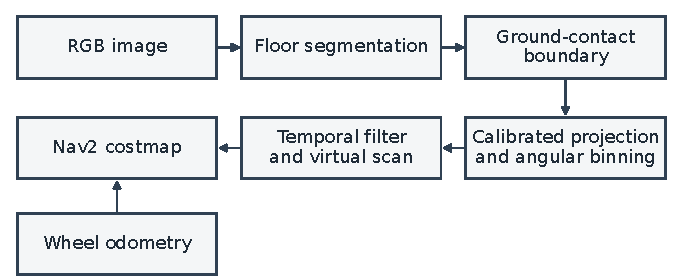
\includegraphics[width=\linewidth]{pipeline.pdf}
  \caption{V-LiDAR system architecture illustrated with a bridge pilot. (a) The recorded RGB image and its offline-replayed floor mask. Dashed guides mark the scan band and the highlighted pixel column. A side-view schematic shows the calibrated projection. (b) The filtered scan with the same acquisition timestamp. Amber marks the same angular bin before filtering in (a) and in the recorded scan in (b). (c) The recorded local costmap and path in the robot frame. Darker cells indicate higher cost. (d) Velocity commands and wheel-odometry and transform (TF) feedback}
  \label{fig:pipeline}
\end{figure}

The implementation uses class ID~0 for the floor mask. The OpenVINO export metadata lists \texttt{person} for ID~0 and \texttt{floor} for ID~1. We checked the mapping by replaying RGB frames paired to recorded scans by acquisition timestamp, discarding the first second for filter initialization. With ID~0, all channels matched the recorded scan within $0.1$~mm in 1,055 of 1,057 corridor frames and 390 of 423 bridge frames. Infinite returns were counted as matches when both outputs were infinite. With ID~1, no scan matched in all channels. This check concerns reproduction of the recorded pipeline output. Pixel-level floor annotations were unavailable for these frames.

The saved model metadata records transfer learning with Ultralytics 8.3.4, 100 epochs, batch size 16, and training image size 320. The stored validation summary includes aggregate mask average precision (AP) of 0.802 at an intersection-over-union threshold of 0.50 and 0.562 over thresholds from 0.50 to 0.95. We could not verify the training dataset export or its validation split for this checkpoint. \pending{R3}{Recover the original dataset version, annotation procedure, label map, and split counts.}

\subsection{Calibrated planar projection and visibility}

Let $(u,v)$ be an image pixel with intrinsics $(f_x,f_y,c_x,c_y)$ after resizing. The stored calibration for $640\times480$ images is scaled to the $320\times256$ input grid. For camera height $h$ and downward pitch $\gamma$, the lookup table uses
\begin{align}
 \theta(u) &= \arctan((u-c_x)/f_x), &
 \phi(v) &= \arctan((v-c_y)/f_y), \\
 x(v) &= \frac{h}{\tan(\phi(v)+\gamma)}, &
 r(u,v) &= \frac{x(v)}{\cos\theta(u)} .
\end{align}
The implementation neglects off-axis pitch coupling in this separable projection. It represents the nearest candidate in each angular bin and publishes 141 bins at $0.5^\circ$ increments over a nominal $[-35^\circ,35^\circ]$ span. Regenerating the lookup tables reproduced the stored files byte for byte. The resized intrinsics are $(f_x,f_y,c_x,c_y)=(258.5994,273.6966,159.4597,134.6184)$ pixels. Image columns map to 127 bins, from $-31.5^\circ$ to $+31.5^\circ$.

For the stored lookup table, the configured height and pitch are $h=1.05\m$ and $\gamma=2.0^\circ$. Substituting the last image row into $x(v)$ yields approximately $2.18\m$ at the optical centerline. The radial lower bound at the left and right edge columns is approximately $2.56\m$. Figure~\ref{fig:scan-visibility} shows these geometric limits. Effective detection also depends on object size, bearing, contrast against the floor, and camera pitch changes during motion.

\begin{figure}[htbp]
  \centering
  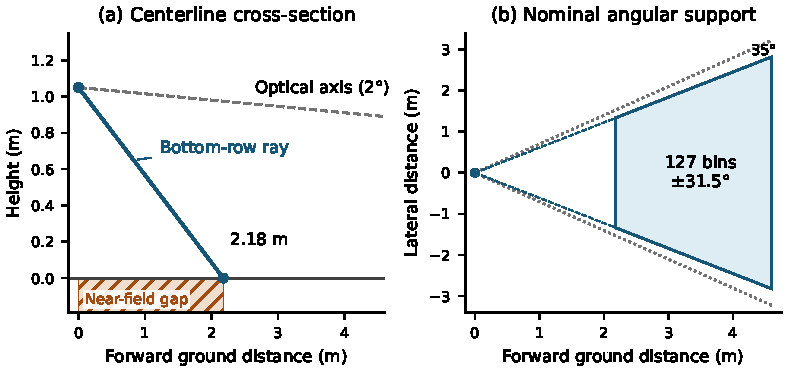
\includegraphics[width=\linewidth]{scan_visibility.pdf}
  \caption{Nominal ground visibility from the stored calibration. (a) The camera's bottom-row ray intersects the ground $2.18\m$ forward at the centerline. (b) The shaded region shows populated angular bins outside the near-field gap. Dotted sides mark the nominal $\pm35^\circ$ scan span. The right boundary is the edge of the drawing}
  \label{fig:scan-visibility}
\end{figure}

For a model-only check, we compared the lookup table against joint ray rotation and intersection with the ground plane at the same configured intrinsics and pose. Within the tabulated $2.18$--$5.00\m$ interval, the maximum differences were below $0.012\m$ in radial range and $0.414^\circ$ in unquantized bearing. The comparison characterizes the separable approximation under the stated model assumptions. The physical mounting and optical origin require independent measurement.

\subsection{Temporal filtering and navigation integration}\label{sec:deployed-setup}

Finite detections are confirmed across two processed frames. A tracked range is smoothed with an exponential moving average ($\alpha=0.6$), and clearing a track also requires two frames. The scan header preserves image acquisition time. Nav2 uses the scan to update its local obstacle map and uses wheel odometry for short-range relative motion. The reference costmap configuration limits ray clearing near the sensor. Whether a high cost persists after ground contact leaves the image depends on prior range observations, robot motion, and costmap updates.

Recorded transforms in the pilot and archived benchmark bags placed the virtual scan frame \texttt{lidar\_link} at $(-0.55,0,0)\m$ relative to \texttt{base\_link}. The RGB header used \texttt{camera\_frame}. The recorded values specify software frames and should be distinguished from the physical optical-center calibration.

The reference Nav2 configuration disables AMCL's transform broadcaster and uses obstacle and inflation layers in the costmaps. The frame bridge supplies the identity transform from \texttt{map} to \texttt{odom} when visual-SLAM poses are absent. All 12,268 recorded \texttt{map}-to-\texttt{odom} transforms across the seven November pilot bags were identities. The recorded wheel-odometry messages used \texttt{odom} as the parent frame and \texttt{base\_footprint} as the child frame.

Figure~\ref{fig:archive-nav2} links a camera frame from a corridor pilot with the corresponding published costmap and local path. The camera shows a box near the left wall. The path lies in the lower-cost region between the higher-cost sides of the corridor.

\begin{figure}[htbp]
  \centering
  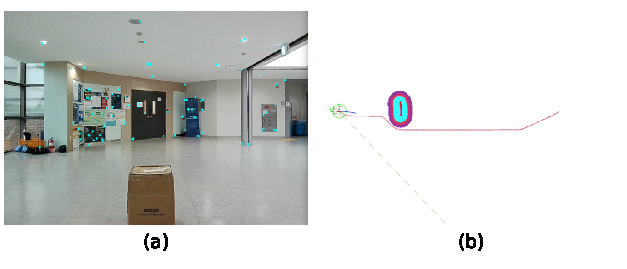
\includegraphics[width=\linewidth]{archive_nav2_view.pdf}
  \caption{Corridor pilot snapshot 37.062~s after recording began. (a) RGB frame sharing the virtual scan's acquisition stamp. (b) Published local costmap and local path displayed relative to the robot. Their recorder times are 61.2 and 36.1~ms after the RGB sample, respectively. Left and right follow the camera view}
  \label{fig:archive-nav2}
\end{figure}

The wheel driver checks freshness of microcontroller velocity feedback. If feedback is stale for 0.25~s, it requests zero velocity and suspends odometry integration. Each formal trial begins after verifying standstill, prior-goal termination, and a fresh reset. \pending{R2}{Record the actual deployed firmware, software revision, camera and scan origins, model and lookup table hashes, and costmap settings used by the formal trials.}

\subsection{Draft preparation}

A large language model assisted in preparing this working manuscript and cross-checking repository documentation. The authors should verify the description, source data, results, and interpretation before submission.

\section{Evaluation protocol}\label{sec:evaluation}

\subsection{Robot trials and outcomes}

The proposed evaluation uses three locations and four conditions. The reference hall from the earlier evaluation is revisited during the day and at night. The other settings provide a corridor with predominantly artificial light and an enclosed bridge with daylight. Floor properties, corridor widths, camera frames, time of day, and obstacle positions document the conditions. Several environmental factors can co-vary between sites. These trials assess performance under those observed combinations.

\ifformalsites
Figure~\ref{fig:site-views} shows forward-facing camera frames with the target obstacles visible in the four formal conditions.
\else
Figure~\ref{fig:site-views} illustrates the planned settings with an earlier setup photograph and available pilot camera frames.
\fi
\begin{figure}[htbp]
  \centering
  \ifformalsites
    \includegraphics[width=\linewidth]{formal_sites.pdf}
    \caption{Forward camera frames from the formal trial recordings. (a) Reference hall by day. (b) Reference hall at night. (c) Artificial-light interior. (d) Daylit bridge}
  \else
    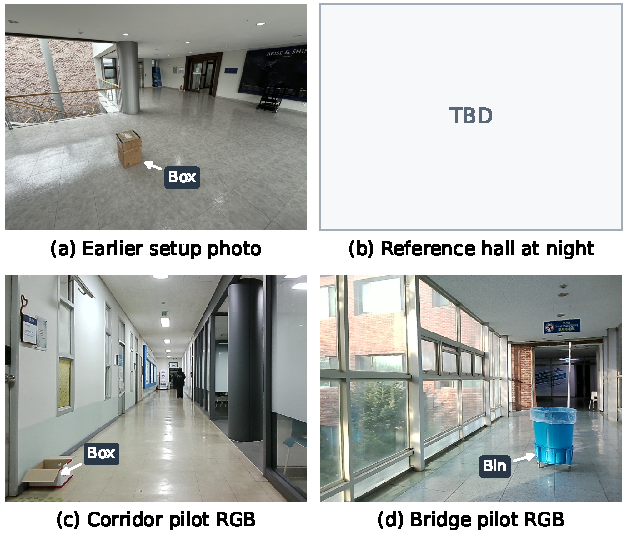
\includegraphics[width=\linewidth]{site_views_draft.pdf}
    \caption{Preview of the four planned settings. (a) Earlier daytime setup photograph of the reference hall. (b) Night view of the reference hall pending. (c) Pilot camera frame from the candidate corridor for the artificial-light condition. (d) Pilot camera frame from the daylit bridge. Arrows identify the objects in the available views}
  \fi
  \label{fig:site-views}
\end{figure}

At each location, the straight-line displacement between marked start and goal locations is 10~m. The obstacle layouts use a box alone and the same box with a chair. Obstacles, starting pose, limits, and navigation settings are fixed and logged. Primary success is physical entry into the marked goal region within the trial time limit, without obstacle contact or manual intervention. A field observer or external video supplies these labels. Nav2 status, time from goal acceptance, trajectory, and message logs provide secondary diagnostics. Report success as a count over all eligible attempts for each condition, with uncertainty and reasons for unusable recordings. Preserve failed attempts and separately identify invalid measurements using documented reasons.

To examine failure causes, review image and scan timestamps, whether an obstacle was represented before the avoidance maneuver, the generated path, and feedback during execution. Compare these timelines for successful and failed attempts. Classify failures as perception, planning, execution, or undetermined when the available signals support that decision. The location of detection and the lowest lateral distance inferred from odometry are diagnostic estimates and depend on the quality of that odometry.

\pending{R1}{Verify the observed outcomes and the corresponding recording IDs for each trial.}
\pending{R2}{Confirm the goal-region dimensions, time limit, and measured obstacle positions.}

\subsection{Scan updates and recorder timing}

For the seven November 26 pilot recordings, we computed scan update rates from the number and span of distinct nonzero acquisition timestamps. We paired virtual scans with RGB frames by identical acquisition timestamps and used the first recorded scan for each source stamp. For each unique match, we subtracted the RGB recorder timestamp from the scan recorder timestamp. The signed difference characterizes the order and spacing with which the two topics reached the recorder. Scan update rate and recorder timing describe different aspects of the system. The timing measurement ends at the recorder and excludes downstream costmap integration and controller response.

\subsection{Offline perception comparison}

A historical replay uses two archived robot recordings from a hall with reflective flooring. The images show a stationary cardboard box in both runs. The analysis compares \vlidar{}, MiDaS v2.1 Small, and Depth Anything V2 Small on the same sampled images. We repeat the comparison on an Intel Core Ultra 7 155H with four PyTorch CPU threads and use each model's native preprocessing. A separate V-LiDAR OpenVINO pass uses the deployment model export. Timing covers the perception wrapper before bearing-window lookup and distance calibration. We exclude the first frame of each bag and run each model in a separate loop.

\subsection{Temporal filter ablation}

We replayed two stationary clips and the navigation intervals of the first two bridge pilots. The stationary clips were the first 12~s of a bridge precheck and of the first reflective-hall recording used in the historical comparison. Wheel odometry reported a fixed pose and zero linear and angular velocity in both stationary clips. We sampled at most one RGB frame per 100~ms bin for the stationary clips. For the moving clips, we used only RGB frames whose acquisition timestamps matched a recorded virtual scan. The Nav2 navigation start and completion log times delimit the moving intervals. We replayed one second before each moving interval to initialize the filter and omitted the first second of the stationary clips.

The same segmentation outputs and range lookup table supplied both the bypass and the temporal filter. We counted validity transitions for each angular channel and computed the mean absolute range step across adjacent frames with valid returns in both configurations at both times. A valid return was finite and within the configured $0.1$--$10$~m scan bounds. For the moving clips, we also examined onsets for which a channel became valid with the bypass and remained invalid with the filter. When the channel was valid in both configurations on the next sampled frame, we used the acquisition timestamp difference to measure the confirmation delay.

\section{Results}\label{sec:results}

\subsection{Formal navigation outcomes}\label{sec:formal-outcomes}

\IfFileExists{formal_trial_rows.tex}{
The condition-level outcomes for the selected configuration are reported in Table~\ref{tab:formal-navigation}.
\begin{table}[htbp]
  \caption{Physical navigation outcomes by condition and obstacle layout. Success is reported as successes over evaluated attempts with a descriptive 95\% Wilson interval. The total number of attempts $N$ includes invalid and unresolved attempts. A dash indicates unavailable data.}
  \label{tab:formal-navigation}
  \centering
  \small
  \setlength{\tabcolsep}{3pt}
  \begin{tabular}{@{}llrrrrr@{}}
  \toprule
  Environment & Layout & $N$ & Success & 95\% CI & Invalid & Pending \\
  \midrule
  \input{formal_trial_rows.tex}
  \end{tabular}
\end{table}
\ifdefined\JINTFormalOutcomesFigure
Figure~\ref{fig:formal-outcomes} shows the success estimates and their descriptive uncertainty.
\begin{figure}[htbp]
  \centering
  \includegraphics[width=\linewidth]{\JINTFormalOutcomesFigure}
  \caption{Physical avoidance success by condition and obstacle layout. Points show success among evaluated attempts and lines show descriptive 95\% Wilson intervals. Fractions give successful over evaluated attempts. ``n/a'' indicates an unrecorded group and ``0 eval.'' indicates that recorded attempts remained invalid or unadjudicated}
  \label{fig:formal-outcomes}
\end{figure}
\fi
\loadtrialsequence{formal_trial_sequence}
\loadtrialsequence{formal_trial_sequence_2}
}{
  Formal trial outcomes are pending.
  \pending{R1}{Insert verified formal trials from the field log.}
}

\pending{R4}{Report the observed pattern across conditions and layouts, and illustrate a representative success and failure if available.}

\subsection{Exploratory bridge trials}

A pair of archived bridge bags shows the robot passing a stationary bin. The recorded Nav2 logs show success messages 61.1 and 44.9~s after navigation began, respectively. The trials were recorded before the present reset and wheel feedback changes. No independent physical contact or goal label is recorded for those pilot runs. Figure~\ref{fig:pilot} links three recorded images from the second bag to the nearest recorded odometry poses and shows both paths after alignment to their initial poses. The maximum magnitudes of lateral displacement were 0.51 and 0.56~m relative to each starting heading. The 20 earlier single-hall runs provide additional archived odometry diagnostics in Online Resource~1, Fig.~S3.

In the second bridge pilot, we tracked a fixed $0.25\m$ radius region centered at the median of five earlier scan endpoints projected into the odometry frame (Online Resource~1, Fig.~S6). The last scan with endpoints in this region was recorded at 22.336~s. The image at 23.016~s shows the bin with its base outside the frame. Two cells with the inscribed obstacle cost (99) remained in the published local costmap at 24.697~s, 2.36~s after the last nearby scan return. The contributions of clearing and inflation to the retained costs remain unresolved.

\begin{figure}[htbp]
  \centering
  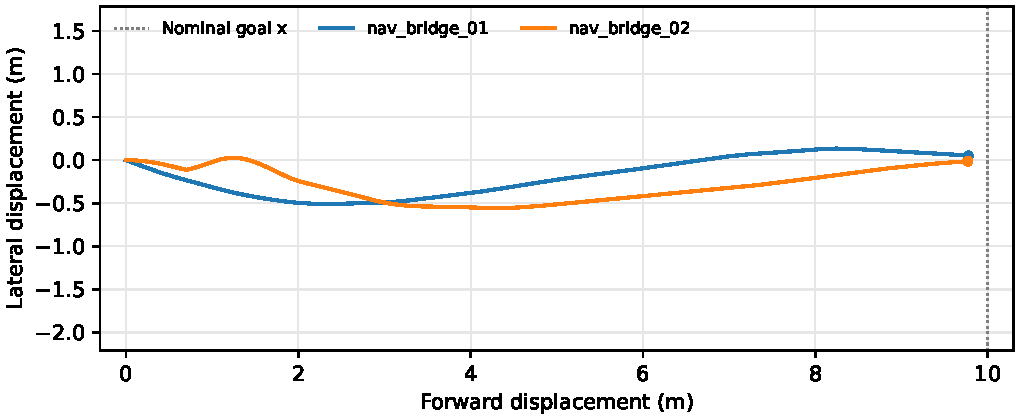
\includegraphics[width=\linewidth]{bridge_pilot_odom.pdf}
  \caption{Exploratory bridge avoidance. Camera frames (a), (b), and (c) come from approximately 10, 25, and 35~s after the start of the second recording. Open markers on the second path mark the nearest poses in recorder time. Filled markers are terminal odometry poses. The dotted line marks the nominal goal displacement. The axes use different scales}
  \label{fig:pilot}
\end{figure}

The third and fourth bridge recordings each contain two global planning failures. In the fifth recording, a new goal preempted the previous goal at 9.28~s from the start of the recording. This event fell within a 15.95~s interval in which the reported odometric forward velocity and yaw rate remained exactly $0.31542$~m/s and $-0.333$~rad/s. Figure~\ref{fig:pilot-diagnostic} compares the recorded scan, commands, and odometry of this run with the second bridge run. At 2.96 and 14.02~s, corresponding features in the two RGB frames moved by a median of less than one pixel while the nearest recorded odometry poses differed by $211^\circ$ in unwrapped yaw (Online Resource~1, Fig.~S4). This discrepancy supports flagging the odometry interval as unreliable. The record leaves open whether the trial would have reached the goal with fresh feedback.

Each of the five planning failures was followed by a global-costmap clear request and a new path to the same logged goal within 91~ms in recorder time. For the second failure in the fourth recording, the last published global costmap preceded the failure by 274~ms. Of the 100 cells centered within $\pm 0.5$~m of the goal along both map axes, 96 had inscribed or lethal costs. A clear request appeared 19~ms after the failure. In the next published grid, 26~ms after the failure, all 100 cells had zero cost. The next global path was recorded 29~ms after the failure (Online Resource~1, Fig.~S5). For the other four failures, the preceding snapshots were 1.74--15.63~s old. The sampled maps leave the planner's exact input state and the physical source of the high costs undetermined.

\begin{figure}[htbp]
  \centering
  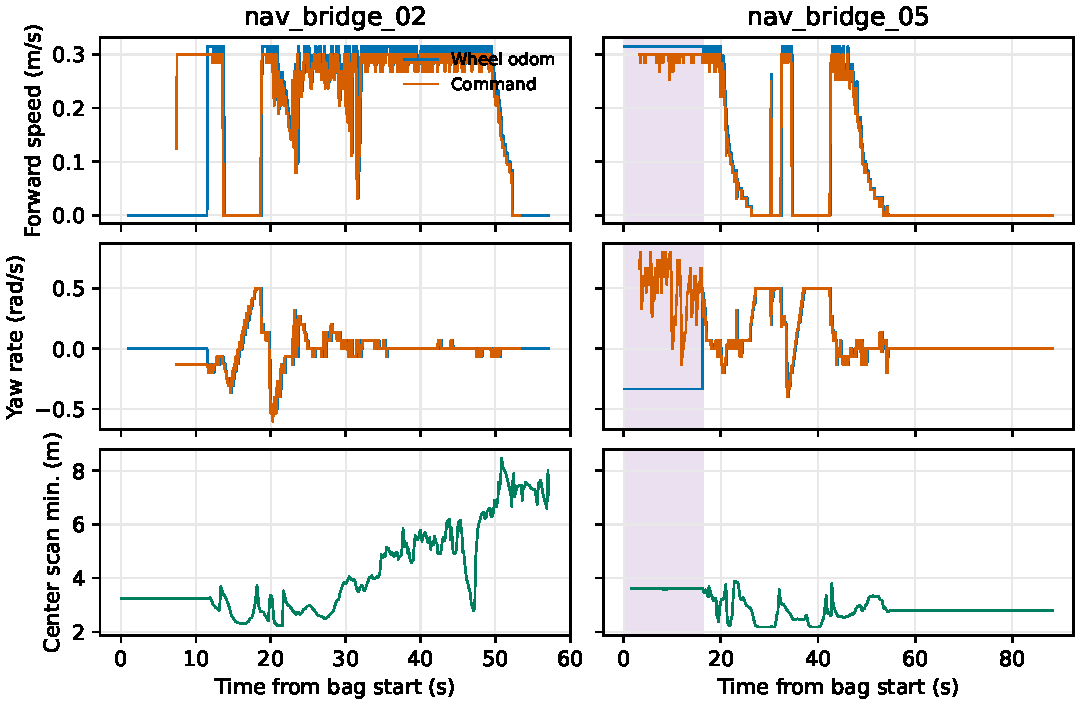
\includegraphics[width=\linewidth]{pilot_command_odometry.pdf}
  \caption{Recorded command and odometry signals for two bridge pilots. The lower traces show the nearest finite virtual-scan range within $10^\circ$ of the center ray. The shaded region marks identical nonzero turning feedback in the fifth recording. The range trace can include surfaces other than the test obstacle}
  \label{fig:pilot-diagnostic}
\end{figure}

\subsection{Recorded scan update rate}

Across all seven pilot recordings, 4,832 of 5,048 distinct nonzero scan timestamps matched unique RGB frames. Mean source update rates ranged from 6.72 to 8.50~Hz. Median update gaps were about 132~ms. The 95th percentile was about 136~ms in six recordings and 300~ms in the remaining recording (Table~\ref{tab:recorder-timing}).

In the five recordings with nonnegative deltas for every matched pair, per-run median recorder deltas ranged from 19.25 to 19.95~ms and per-run 95th percentiles from 22.84 to 24.06~ms. The other two recordings contained pairs whose scan was stored first. These signed recorder deltas characterize recording order. The two older recordings used for the offline perception comparison had no exact camera-to-scan stamp matches.

\begin{table}[htbp]
\caption{Virtual scan update cadence and timestamp matching in the November pilots. Scan-first pairs have negative recorder timestamp differences.}
\label{tab:recorder-timing}
\centering
\begin{tabular}{@{}lrrrr@{}}
\toprule
Pilot & Rate (Hz) & Gap p95 (ms) & Matched / scan & Scan-first pairs \\
\midrule
Hall test & 8.47 & 136 & 1066 / 1066 & 0 \\
Hall rerun & 8.45 & 136 & 775 / 787 & 0 \\
Bridge 01 & 8.45 & 136 & 717 / 717 & 0 \\
Bridge 02 & 8.02 & 136 & 432 / 459 & 30 \\
Bridge 03 & 6.72 & 300 & 314 / 472 & 289 \\
Bridge 04 & 8.44 & 136 & 804 / 810 & 0 \\
Bridge 05 & 8.50 & 136 & 724 / 737 & 0 \\
\bottomrule
\end{tabular}
\end{table}

\subsection{Offline CPU timing}

Table~\ref{tab:timing} presents the repeated comparison on archived RGB. The offline timings use 198 frames after discarding the two initial frames. The empirical distributions are shown in Online Resource~1, Fig.~S2. The PyTorch measurements share a CPU and thread settings. Each system uses its native model input resolution and wrapper, so the timings characterize these implementations. The separate OpenVINO measurement uses the same V-LiDAR input size as the PyTorch pass. Table~\ref{tab:recorder-timing} separately describes virtual scan updates observed during robot operation.

\begin{table}[htbp]
\caption{CPU latency on two archived RGB recordings. Input sizes are height by width. Frames within a recording are temporally correlated.}\label{tab:timing}
\centering
\begin{tabular}{@{}lrrr@{}}
\toprule
Method and backend & Input (px) & Mean (ms) & p95 (ms) \\
\midrule
V-LiDAR, PyTorch & $256 \times 320$ & 20.18 & 22.74 \\
V-LiDAR, OpenVINO FP16 & $256 \times 320$ & 13.49 & 16.80 \\
MiDaS v2.1 Small, PyTorch & $192 \times 256$ & 37.32 & 43.92 \\
Depth Anything V2 Small, PyTorch & $518 \times 686$ & 561.39 & 593.84 \\
\bottomrule
\end{tabular}
\end{table}

\subsection{Temporal filter ablation}\label{sec:filter-results}

For the two stationary clips, enabling the filter reduced the mean adjacent-frame change by 41\% in the bridge precheck and 43\% in the reflective hall on common valid samples (Table~\ref{tab:filter}). During the two bridge pilots, the mean range steps fell by 26\% and 23\%, and validity transitions fell by 43\% and 41\%, respectively. The fraction of valid entries changed by less than 0.4 percentage points in each clip.

In the moving clips, 81 and 58 initially withheld channel onsets were valid in both configurations on the next sampled frame. Their median confirmation delays were 132 and 100~ms, respectively, with a 95th percentile of 136~ms in both clips. Another 109 and 96 initially withheld onsets lasted one bypass frame and were invalid in the filtered output on both frames. Channel observations are correlated. These replays characterize scan stability and confirmation time along the recorded paths. Online Resource~2 provides samples and recalculation scripts for the filter, recorded scan timing, and CPU timing results.

\begin{table}[htbp]
\caption{Paired replay with the temporal filter bypassed and enabled. Range steps use adjacent-frame channel pairs with valid returns in both variants at both times. The four clips have 13,835, 8,945, 60,604, and 40,291 such pairs, respectively.}
\label{tab:filter}
\centering
\begin{tabular}{@{}lrrrrr@{}}
\toprule
& & \multicolumn{2}{c}{Validity transitions} & \multicolumn{2}{c}{Mean range step (cm)} \\
\cmidrule(lr){3-4} \cmidrule(lr){5-6}
Clip & Frames & Bypass & Enabled & Bypass & Enabled \\
\midrule
Bridge precheck & 110 & 8 & 0 & 1.29 & 0.76 \\
Reflective hall & 110 & 50 & 25 & 6.13 & 3.52 \\
Bridge pilot 1 & 518 & 1,624 & 930 & 27.01 & 19.98 \\
Bridge pilot 2 & 350 & 980 & 576 & 22.49 & 17.42 \\
\bottomrule
\end{tabular}
\end{table}

\section{Discussion}\label{sec:discussion}

The virtual scan interface enables the navigation stack to consume observations from monocular floor segmentation. Its operating envelope depends on a forward-facing camera, visible ground contact, and a stable camera-to-base relationship. Floor reflections, strong shadows, low floor-to-object contrast, and pitch variation can degrade the boundary projection. Limited field of view and the ground-contact blind region also constrain the configurations that can be covered. A wheel odometry fault can produce a separate failure even when the camera continues to provide plausible observations.

In the archived scene with a box and window glare (Fig.~\ref{fig:floor-reflection}), offline inference produced an isolated mask above the scan band. The spatial mask-selection rule removed this region. Online Resource~1, Fig.~S1 shows additional archived views of a chair, a cart, glare, and a narrow passage. A temporal filter can suppress a transient return, while a persistent segmentation error can affect consecutive frames. Causally attributing a collision or a failure to avoid therefore requires agreement between the camera, scan, and navigation records.

\begin{figure}[htbp]
  \centering
  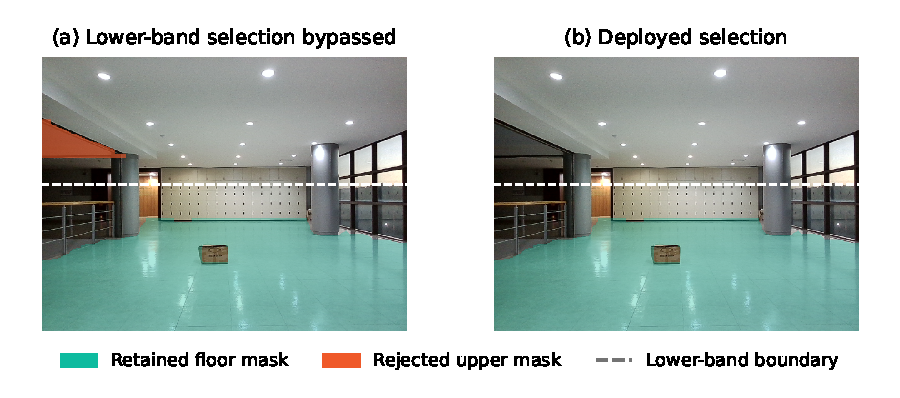
\includegraphics[width=\linewidth]{archive_floor_reflection.pdf}
  \caption{Offline replay of one archived image from a reflective hall. (a) Mask union with lower-band selection bypassed, including a spurious upper region in orange. (b) Mask union with deployed selection. Teal indicates the retained mask, and the dashed line marks the start of the lower scan band}
  \label{fig:floor-reflection}
\end{figure}

The archived nominal obstacle coordinates lack a documented measurement origin. If those coordinates are held fixed in the odometry frame, using the logged virtual scan offset instead of a zero sensor offset changes the nominal reference distances by $0.51$--$0.55\m$ on 59 previously selected frames. This sensitivity shows why absolute range evaluation requires an independently surveyed obstacle reference in the appropriate frame.

The offline comparisons characterize computational cost and scan stability in stationary and moving clips. The physical trials address how the full sensing and control stack behaves in the tested configurations. The ablation leaves the recorded viewpoints unchanged, so it cannot establish a change in closed-loop success or quantify the effect of waiting for confirmation when approaching an obstacle. Cross-site results should be interpreted alongside the observed layouts, floor appearances, and illumination, which can vary together. The protocol focuses on stationary obstacle avoidance with wheel odometry in the stated operating conditions.

\pending{R4}{Tie the operating limits to observed failures and state the uncertainty in their attribution.}

\section{Conclusion}\label{sec:conclusion}

\vlidar{} provides a calibrated planar observation from monocular RGB images for indoor reactive avoidance on a wheeled robot. Archived data support pilot demonstrations and an offline computation comparison. \pending{R4}{Conclude using observed condition-level performance and observed limits after verification of the formal trials.}

\bmhead{Supplementary information}
Online Resource~1 contains selected archived camera frames, empirical CPU timing distributions, terminal odometry diagnostics, an image--odometry comparison, a global-costmap comparison around a planning failure, and a local-costmap trace around earlier scan observations.

Online Resource~2 contains per-frame CPU timings, relative scan and camera timestamps, paired filter replay arrays, and scripts to recalculate the numerical summaries.

\bibliography{references}

\section*{Statements and Declarations}
\label{sec:declarations}

\textbf{Funding.} The funding statement is pending confirmation. \pending{R5}{Check which awards from the IEEE draft (2026-ANCHOR-15-119, RS-2025-24683458, and 202500590001) supported this work.}

\noindent\textbf{Competing interests.} The disclosure is pending confirmation. \pending{R5}{Confirm the competing interests statement with the coauthors.}

\noindent\textbf{Data availability.} Numerical samples and aggregation scripts for the CPU timing, scan cadence, and temporal-filter results are included in Online Resource~2. Access details for trial outcomes, setup records, and raw sensor recordings are pending confirmation. \pending{R6}{Insert the verified archive location and access terms for trial records and footage.}

\noindent\textbf{Author contributions.} All authors contributed equally to this work.

\end{document}
